\documentclass[10pt]{article}

\usepackage{amsmath}
\usepackage{amsthm}
\usepackage{amssymb}
\usepackage[pdftex]{graphicx}
\usepackage{subfig}
\usepackage{wrapfig}
\usepackage{enumerate}
\usepackage{fancyhdr}
\usepackage{listings}
\usepackage{textcomp}
\usepackage[
  pdftitle={},%
  pdfauthor={},%
  pdfsubject={},%
  pdfkeywords={},%
  pdfstartview=FitH,%
  bookmarks=true,%
  bookmarksopen=true,%
  breaklinks=true,%
  colorlinks=true,%
  linkcolor=red,anchorcolor=black,%
  citecolor=green,filecolor=cyan,%
  menucolor=red,urlcolor=magenta,%
  pdftex]{hyperref}
\usepackage{makeidx}
\usepackage{subfig}
\usepackage{wrapfig}
\usepackage[usenames]{color}
\usepackage[sectionbib]{chapterbib}
\usepackage[square,numbers,sort&compress,sectionbib,nonamebreak]{natbib}
\usepackage[margin=1.0in,a4paper,portrait]{geometry}
\usepackage[Bjarne]{fncychap}
\usepackage{minitoc} 
\usepackage{float}
\usepackage{tikz}
\usepackage{multirow}
\makeindex

\renewcommand\familydefault{\sfdefault}

%\usepackage{../../styles/clrscode3e}
%\usepackage{../../styles/clrmac}
%\usepackage{../../styles/supertech-sig}

%%%%%%%%%% Start TeXmacs macros
% macro for todo entries
%The first argument is the name of the person who should do the specified tak. This argument is optional and defaults to ``scribe''. 
%The second argument describes the type of the task. Tasks can be 
%missing 
%expand 
%clarify 
%reference 
%incorrect 
%editing 

%The third argument contains the message describing what needs to be done. 
\definecolor{CornSilk}{rgb}{1,1,.88}
\newcommand{\todo}[3][scribe]{\textbf{\textcolor{red}{TODO: #2}} \textit{\textcolor{green}{@#1}\textcolor{blue}{ : #3}}}
%aside note: 
\newcommand{\sidenote}[1]{\fcolorbox{black}{CornSilk}{\parbox{6 in}{\textit{\textbf{\Large{Did You Know?}}}\newline #1}}}
\newcommand{\nbdiscussion}[1]{\footnote{\fcolorbox{black}{CornSilk}{\parbox{6 in}{\textit{\textbf{\Large{NB Discussion}}}\newline #1}}}}
\newcommand{\faq}[2]{\fcolorbox{black}{CornSilk}{\parbox{6 in}{\textbf{\textit{\Large{FAQ}}}\newline 
\begin{description} 
\item[\textbf{Q:}] #1
\newline 
\item[\textbf{A:}] #2
\end{description} }}}
\newcommand{\hilight}[1]{\colorbox{yellow}{#1}}
\newcommand{\tmabbr}[1]{#1}
\newcommand{\tmem}[1]{{\em #1\/}}
\newcommand{\tmop}[1]{\ensuremath{\operatorname{#1}}}
\newcommand{\tmstrong}[1]{\textbf{#1}}
\newcommand{\tmtextit}[1]{{\itshape{#1}}}
\newcommand{\tmtexttt}[1]{{\ttfamily{#1}}}
\newcommand{\getdir}{images}
\newcommand{\keyword}[1]{\index{#1|textbf}}
\newcommand{\mainword}[1]{\textbf{#1}}
\newenvironment{enumeratenumeric}{\begin{enumerate}[1.] }{\end{enumerate}}
\newenvironment{itemizedot}{\begin{itemize} \renewcommand{\labelitemi}{$\bullet$}\renewcommand{\labelitemii}{$\bullet$}\renewcommand{\labelitemiii}{$\bullet$}\renewcommand{\labelitemiv}{$\bullet$}}{\end{itemize}}
\newenvironment{tmparsep}[1]{\begingroup\setlength{\parskip}{#1}}{\endgroup}

 %%%%%%%%%% End TeXmacs macros

%set the margins to a reasonable value 
%\addtolength{\oddsidemargin}{-.75in}
%\addtolength{\evensidemargin}{-.75in}
%\addtolength{\textwidth}{1.5in}
%\addtolength{\topmargin}{-.875in}
%\addtolength{\textheight}{1.75in}

\usepackage{calc}

\makeatletter
\newcommand{\DESCRIPTION@original@item}{}
\let\DESCRIPTION@original@item\item
\newcommand*{\DESCRIPTION@envir}{DESCRIPTION}
\newlength{\DESCRIPTION@totalleftmargin}
\newlength{\DESCRIPTION@linewidth}
\newcommand{\DESCRIPTION@makelabel}[1]{\llap{#1}}%
\newcommand{\DESCRIPTION@item}[1][]{%
  \setlength{\@totalleftmargin}%
       {\DESCRIPTION@totalleftmargin+\widthof{\textbf{#1 }}-\leftmargin}%
  \setlength{\linewidth}
       {\DESCRIPTION@linewidth-\widthof{\textbf{#1 }}+\leftmargin}%
  \par\parshape \@ne \@totalleftmargin \linewidth
  \DESCRIPTION@original@item[\textbf{#1}]%
}
\newenvironment{DESCRIPTION}
  {\list{}{\setlength{\labelwidth}{0cm}%
           \let\makelabel\DESCRIPTION@makelabel}%
   \setlength{\DESCRIPTION@totalleftmargin}{\@totalleftmargin}%
   \setlength{\DESCRIPTION@linewidth}{\linewidth}%
   \renewcommand{\item}{\ifx\@currenvir\DESCRIPTION@envir
                           \expandafter\DESCRIPTION@item
                        \else
                           \expandafter\DESCRIPTION@original@item
                        \fi}}
  {\endlist}
\makeatother

% Macros for proofs, theorems, etc.
\theoremstyle{plain}% default
\newtheorem{thm}{Theorem}[section]
\newtheorem{lem}[thm]{Lemma}
\newtheorem{prop}[thm]{Proposition}
\newtheorem*{cor}{Corollary}
\newtheorem*{KL}{Klein’s Lemma}
\theoremstyle{definition}
\newtheorem{defn}{Definition}[section]
\newtheorem{conj}{Conjecture}[section]
\newtheorem{exmp}{Example}[section]
\theoremstyle{remark}
\newtheorem*{rem}{Remark}
\newtheorem*{note}{Note}
\newtheorem{case}{Case}

\newenvironment{definition}[1][Definition]{\begin{trivlist}
\item[\hskip \labelsep {\bfseries #1}]}{\end{trivlist}}
\newenvironment{example}[1][Example]{\begin{trivlist}
\item[\hskip \labelsep {\bfseries #1}]}{\end{trivlist}}
\newenvironment{remark}[1][Remark]{\begin{trivlist}
\item[\hskip \labelsep {\bfseries #1}]}{\end{trivlist}}



\begin{document}

\title{{\small 6.830 Term Project - Spring 2013}\\Machine Learning Algorithms for In-Database Analytics}
\author{Franck Dernoncourt \& Sumaiya Nazeen}
\maketitle 

\abstract{Our project focused on extending the functionality of MADlib. MADlib is an open source machine learning and statistics library which works with Postgres or Greenplum to provide in-database analytics. Although some machine learning algorithms have been implemented in MADlib, there is room for additional contributions. We implemented two different machine learning algorithms, symbolic regression with genetic programming and adaptive boosting for MADlib, and are in the process of contributing our code to the MADlib community codebase. We also assess the performance of our implementations and compare their performance with the same algorithms outside MADlib.}

\section{Introduction}
\label{sect:introduction}
Traditionally, large databases were mainly used for {\itshape data warehousing} i.e. accounting purposes in enterprises, supporting financial record-keeping and reporting at various levels of granularity. However, over the past decade, attitudes toward large databases have been changing quickly. Focus of large database usage has shifted from accountancy to analytics. Though the need for correct accounting and data warehousing practice still prevails, but it is becoming a shrinking fraction of the volume. The emerging trend rather focuses on supporting predictive analytics via statistical models and algorithms, for potentially noisy data.

In 2008, a group of data scientists came together to describe the emerging trend in database industry and developed a number of non-trivial analytics techniques implemented as simple SQL scripts~\cite{mad09}. They called it MAD, an acronym for \emph{Magnetic} platform, \emph{Agile} design patterns for modeling, loading and iterating over data, and \emph{Deep} statistical models and algorithms for data analysis. This work eventually led to the development of a software framework - a library of analytic methods that can be installed and executed within a relational database engine that supports extensible SQL~\cite{madlib12}. This library is known as MADlib.

MADlib is a free, open source library for in database analytic method available at \url{http://madlib.net}. It provides an evolving suite of SQL-based algorithms for machine learning, data-mining and statistics that run at scale within a database engine, with no need for data import/export to other tools. The goal of MADlib project is to eventually serve a role for scalable database systems that is similar to the CRAN library for R: a community repository of statistical methods supporting scalability and parallelism. At present, MADlib works with Postgres and Greenplum only and provides support for a limited set of analytic methods as shown in Table~\ref{tab:mad}. The methods are implemented mostly in python, C++ and SQL. The project is open for contributions of both new methods, and ports to additional database platforms.

\begin{table}[!ht]
\centering
\begin{tabular}{|l|l|}
\hline
Category & Method\\
\hline
Supervised Learning & Linear Regression\\
& Logistic Regression\\
& Naive Bayes Classification\\
& Decision Trees (C4.5)\\
& Support Vector Machines\\
\hline
Unsupervised Learning & k-Means Clustering\\
& SVD Matrix Factorization\\
& Latent Dirichlet Allocation\\
& Association Rules\\
\hline
Descriptive Statistics & Count-Min Sketch\\
& Flajolet-Martin Sketch\\
& Data Profiling\\
& Quantiles\\
\hline
Support Modules & Sparse Vectors\\
& Array Operations\\
& Conjugate Gradient Optimization\\
\hline
\end{tabular}
\caption{Methods provided in MADlib v0.3~\cite{madlib12}}
\label{tab:mad}
\end{table}

In this project, we aimed at contributing to the MADlib project by implementing two different machine learning algorithms - the first one is {\itshape Genetic Programming} which is a prediction algorithm and the second one is {\itshape Adaptive Boosting} which is a popular classification algorithm. Our goal was to implement those algorithms in python and SQL, incorporate them into MADLib and analyze their performance on a number of factors.

The rest of the report is organized as follows: in Section~\ref{sec:relwork} we discuss the state of the art. Section~\ref{sec:imp}, describes the background for each of the algorithms we implemented. We also discuss the MADlib implementations of the algorithms. In Section~\ref{sec:bench}, we discuss the benchmarking setup and datasets. We also discuss our findings from benchmarking the algorithms on various factors. Finally, we conclude our report in Section~\ref{sec:con}.

\section{Related Works}
\label{sec:relwork}
The space of approaches that combines analytics with data has been growing rapidly. At a high level, there are two approaches:
\begin{enumerate}
\item Top-down language-based approach: This approach brings a statistical language to a data processing substrate.
\item Framework-based approach: This approach provides a framework to express statistical techniques on top of a data processing substrate. 
\end{enumerate}
  
Top-down approaches begin with a high-level statistical programming language like R or Matlab to specify machine learning algorithms. These high-level algorithms are then compiled down to the data infrastructure. Examples of such approach are System ML from IBM~\cite{systemml11}, Revolution Analytics~\cite{rev} and SNOW~\cite{snow09}.

Framework-based approaches provide a set of building blocks (individual machine learning algorithms) with library support for macro- and micro-programming to write the algorithms. Typically they provide a template to automate the common aspects of deploying an analytic task over a data substrate. There have been different framework based approaches for different data substrates. For example, MADlib provides a machine learning and statistics library for RDBMS~\cite{madlib12}. Apache Mahout provides an open source machine learning library for Apache Hadoop~\cite{mahout}. SciDB advocates a completely rewritten DBMS engine for numerical computation~\cite{scidb11}. GraphLab framework provides simplified support for programming parallel machine learning tasks~\cite{graph12}. Spark is a Scala-based domain-specific language (DSL) targeted at machine learning, providing access to the fault-tolerant, main-memory resilient distributed datasets~\cite{resi12}. ScalOps provides a Scala DSL for machine learning that is translated to Datalog, which is then optimized to run in parallel on the Hyracks infrastructure~\cite{hyracks11}. ScalOps bears more similarity with MADlib since it has its origins in Datalog and parallel relational algebra.

We limited our focus on understanding and extending MADlib. Currently, MADlib has much room for growth in multiple dimensions. The MADlib library supports only a limited number of machine learning algorithms as shown in Table~\ref{tab:mad}. So, there is an open invitation to contribute additional statistical models and algorithmic methods, both textbook techniques and cutting-edge research. Also, there is the challenge of porting MADlib to DBMSs other than PostgreSQL and Greenplum. Since MADlib is open source, anyone can contribute to MADlib codebase following their guidelines. 

\section{Implementation of Algorithms}
\label{sec:imp}
In this section, we discuss the implementation details of our algorithm. Before diving into the details of our implementations, first we look at the architecture of MADlib. Then we discuss the background and implementation details of genetic programming and adaptive boosting.
\subsection{Understanding MADlib architecture}
Performing linear algebra over matrices is at the heart of many statistical methods.And it is quite challenging for relational databases to operate over very large matrices. At a macroscopic scale, the matrices need to be partitioned intelligently so that the partitions can be fit into memory of a single machine and then there should be options for movement of these partitions in and out of database by using SQL constructs. At microscopic level, the database engine needs to be able to invoke efficient linear algebra functions on the data partitions. MADlib uses a number of techniques to address these challenges:

\subsubsection*{User-defined Aggregation}
MADlib uses user-defined aggregates (UDA) as a basic building block in the macroscopic level whenever applicable. UDAs are the natural way in SQL to implement mathematical functions that take arbitrary number of tuples as input. A user-defined aggregate consists of three user-defined functions:
\begin{itemize}
\item A {\it transition function} that takes current transition state and a new tuple and combines them into a new transition state.
\item An optional {\it merge function} that takes two transition states and computes a new combined transition state. This function is only needed for parallel execution.
\item A {\it final function} that takes a transition state and transforms it into output value.
\end{itemize}

However, UDAs are not enough for implementing iterative algorithms which perform multiple passes over the data.

\subsubsection*{Driver functions for Multipass Iteration}
Many statistical and machine learning algorithms are iterative in nature and do multiple passes over the dataset. They cannot be implemented as simple UDAs. MADlib implements complex iterative methods by writing driver user-defined functions (UDF) in Python to control iteration. The driver UDF stores any inter-iteration output into a temporary table and reuses the resulting table in subsequent iterations as needed. Final outputs are also stored in tables unless they are small, and can be queried as needed. As a result all data movement is done inside database engine and its bufferpool.

\subsubsection*{Support for Microprogramming}
MADlib implements row-level UDFs (functions that are called multiple times per row) in C or C++. Thus, these functions can call open source libraries like LAPACK or Eigen. MADlib also includes a sparse matrix library written in C.

\subsubsection*{C++ abstraction layer for UDFs} 
MADlib provides a C++ abstraction layer for making it easier to write driver UDFs. UDFs can be written using standard C++ atomic types as well as vector and matrix types that are native to linear algebra operations. The C++ abstraction layer also provides memory management and exception handling support. Finally, it includes third-party libraries so that developers can write efficient code.

\subsubsection*{Python support for UDFs}
MADlib is still in its early stages of development. So it does not provide a full-fledged Python abstraction layer for writing driver UDFs. It only provides a database access layer via {\ttfamily plpy.py} module. PostrgreSQL PL/Python language currently uses an internal plpy.py module to implement seamless DB access (using classic PyGreSQL interface, pg). The python abstraction layer is still under development.

Currently, most of the MADlib functions require to be cognizant of the schema of the input tables and produce output table with fixed schema. 

\subsection{Genetic Programming for symbolic regression}
\subsubsection{Background}

Genetic programming is a subset of evolutionary algorithms, which is a family of optimization algorithms based on the principle of \textbf{Darwinian natural selection}. As part of natural selection, a given environment has a population of individuals that compete for survival and reproduction. The ability of each individual to achieve these goals determines their chance to have children, in other words to pass on their genes to the next generation of individuals, who for genetic reasons will have an increased chance of doing well, even better, in realizing these two objectives.

~~\\
This principle of continuous improvement over the generations is taken by evolutionary algorithms to optimize solutions to a problem. In the \textbf {initial generation}, a \textbf{population} composed of different \textbf {individuals} is generated randomly or by other methods. An individual is a solution to the problem, more or less good: the quality of the individual in regards to the problem is called \textbf{fitness}, which reflects the adequacy of the solution to the problem to be solved. The higher the fitness of an individual, the higher it is likely to pass some or all of its genotype to the individuals of the next generation.

~~\\
An individual is coded as a \textbf{genotype}, which can have any shape, such as a string (genetic algorithms), a vector of real (evolution strategies) or in our case a tree (genetic programming). Each genotype is transformed into a \textbf{phenotype} when assessing the individual, i.e. when its fitness is calculated. In some cases, the phenotype is identical to the genotype: it is called \textbf{direct coding}. Otherwise, the coding is called indirect. For example, suppose you want to optimize the size of a rectangular parallelepiped defined by its length, height and width. To simplify the example, assume that these three quantities are integers between 0 and 15. We can then describe each of them using a 4-bit binary number. An example of a potential solution may be to genotype 0001 0111 01010. The corresponding phenotype is a parallelepiped of length 1, height 7 and width 10.

~~\\
During the transition from the old to the new generation are called \textbf{variation operators}, whose purpose is to manipulate individuals. There are two distinct types of variation operators:
\begin{itemize}
	\item the \textbf{mutation operators}, which are used to introduce variations within the same individual, as genetic mutations;
	\item the \textbf{crossover operators}, which are used to cross at least two different genotypes, as genetic crosses from breeding.
\end{itemize}

The figure \ref{fig:algorithmes_evolutionnistes_synopsis} summarizes how an evolutionary algorithm works.

\begin{figure}[htb]
	\centering
		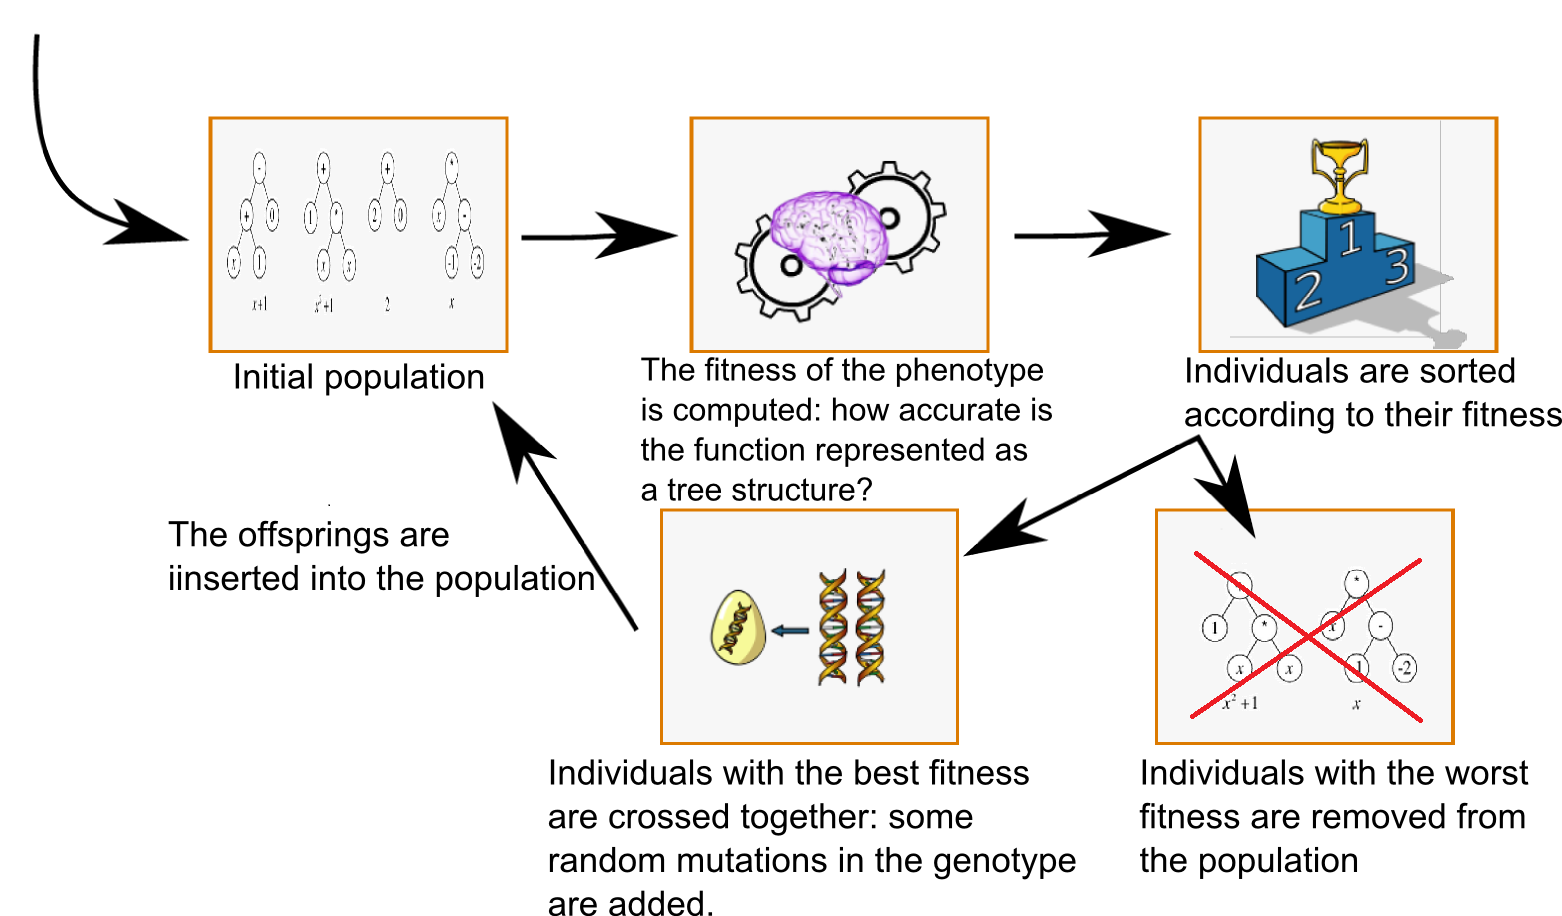
\includegraphics[width=0.8\textwidth]{genetic_programming_regression_synopsis.png}
	\caption[Functioning of an evolutionary algorithm]{Functioning of an evolutionary algorithm: from an initial population of solutions (in symbolic regression, a solution is the tree representing a fraction), they are ranked according to their fitness, the worst ones are eliminated and the best ones are used to produce new solutions.}
	\label{fig:algorithmes_evolutionnistes_synopsis}
\end{figure}

\begin{figure}[htb]
	\centering	
		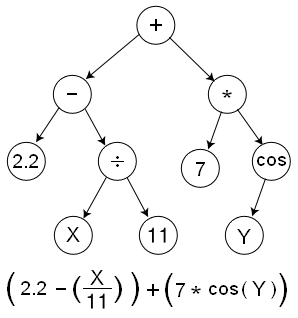
\includegraphics[scale=0.45]{Genetic_Program_Tree.png}
	\caption[A function represented as a tree structure.]{A function represented as a tree structure. Source: Wikipedia}
	\label{fig:Genetic_Program_Tree}
\end{figure}

~~\\
Genetic programming is a perfect suit for symbolic regression. The term "symbolic regression" represents the process during which measured data are fitted by suitable mathematical formula like $x^2 + C$, $sin(x) + 1/e^x$,  etc. The figure \ref{fig:Genetic_Program_Tree} shows how a formula can the represented as a tree. This process is quite well known amongst mathematician and is used when some data of unknown process are obtained. The domain of symbolic regression is of functional nature, i.e. it consists of a function set like ($sin()$, $cos()$, $gamma()$, $MyFunction()$,...) and so called terminal set ($t$, $x$, $p$, ...). The final program is synthesized from a mixture of both sets, and can be quite complicated from a structural point of view. We plan to use genetic programming for symbolic regression in order to unravel unknown relation between some given attributes of a relation. 


\subsubsection{Madlib Implementation}
We implemented the symbolic regression using genetic programming within a Python module for MADlib that depends on the Python evolutionary computation framework DEAP ~\cite{DEAPJMLR2012}. The user can choose whether to store the data in memory, or retrieve by batch: this is a CPU vs. RAM trade-off.

~~\\
Below is an example of a query that runs a symbolic regression, with 100 individuals per population size, 20 generations, and with a maximum size of the trees of 3. It takes 3 attributes as input (x1, x2 and x3) and one attribute as output (y1):

\begin{verbatim}
postgres=# SELECT * from madlib.gp('mock', '{x1, x2, x3}', '{y1}', 100, 20, 3);
\end{verbatim}

\subsection{Adaptive Boosting}
\subsubsection{Background}
Boosting is one of the most important developments in classification methodology. Boosting works by iteratively applying a classification algorithm to re-weighted versions of the training data and then taking a weighted majority vote of the sequence of classifiers thus produced. For many classification algorithms, this simple strategy results in dramatic improvements in performance. While boosting has evolved over the years, we focus on the most commonly used version of boosting known as Adaptive Boosting (AdaBoost) for binary classification developed by Freund and Schapire~\cite{boost96}.

Let us look at a concise description of AdaBoost in a two-class classification setting. We have training data $(x_1, y_1), \ldots, (x_n, y_n)$ with $x_i$ a vector valued feature and $y_i = -1\text{ or }1$. We define $F(x) = \sum_1^M{c_mf_m(x)}$ where each $f_m(x)$ is a classifier producing values $1\text{ or }-1$ and $c_m$ are constants; the corresponding prediction is $\text{sign}(F(x))$. The AdaBoost procedure trains the classifiers $f_m(x)$ on weighted versions of the training sample, giving higher weight to cases that are currently misclassified. This is done for a sequence of weighted samples, and then the final classifier is a linear combination of the classifiers from each stage. The pseudocode for AdaBoost is given in Figure~\ref{fig:adaproc}.

\begin{figure}[ht]
\centering
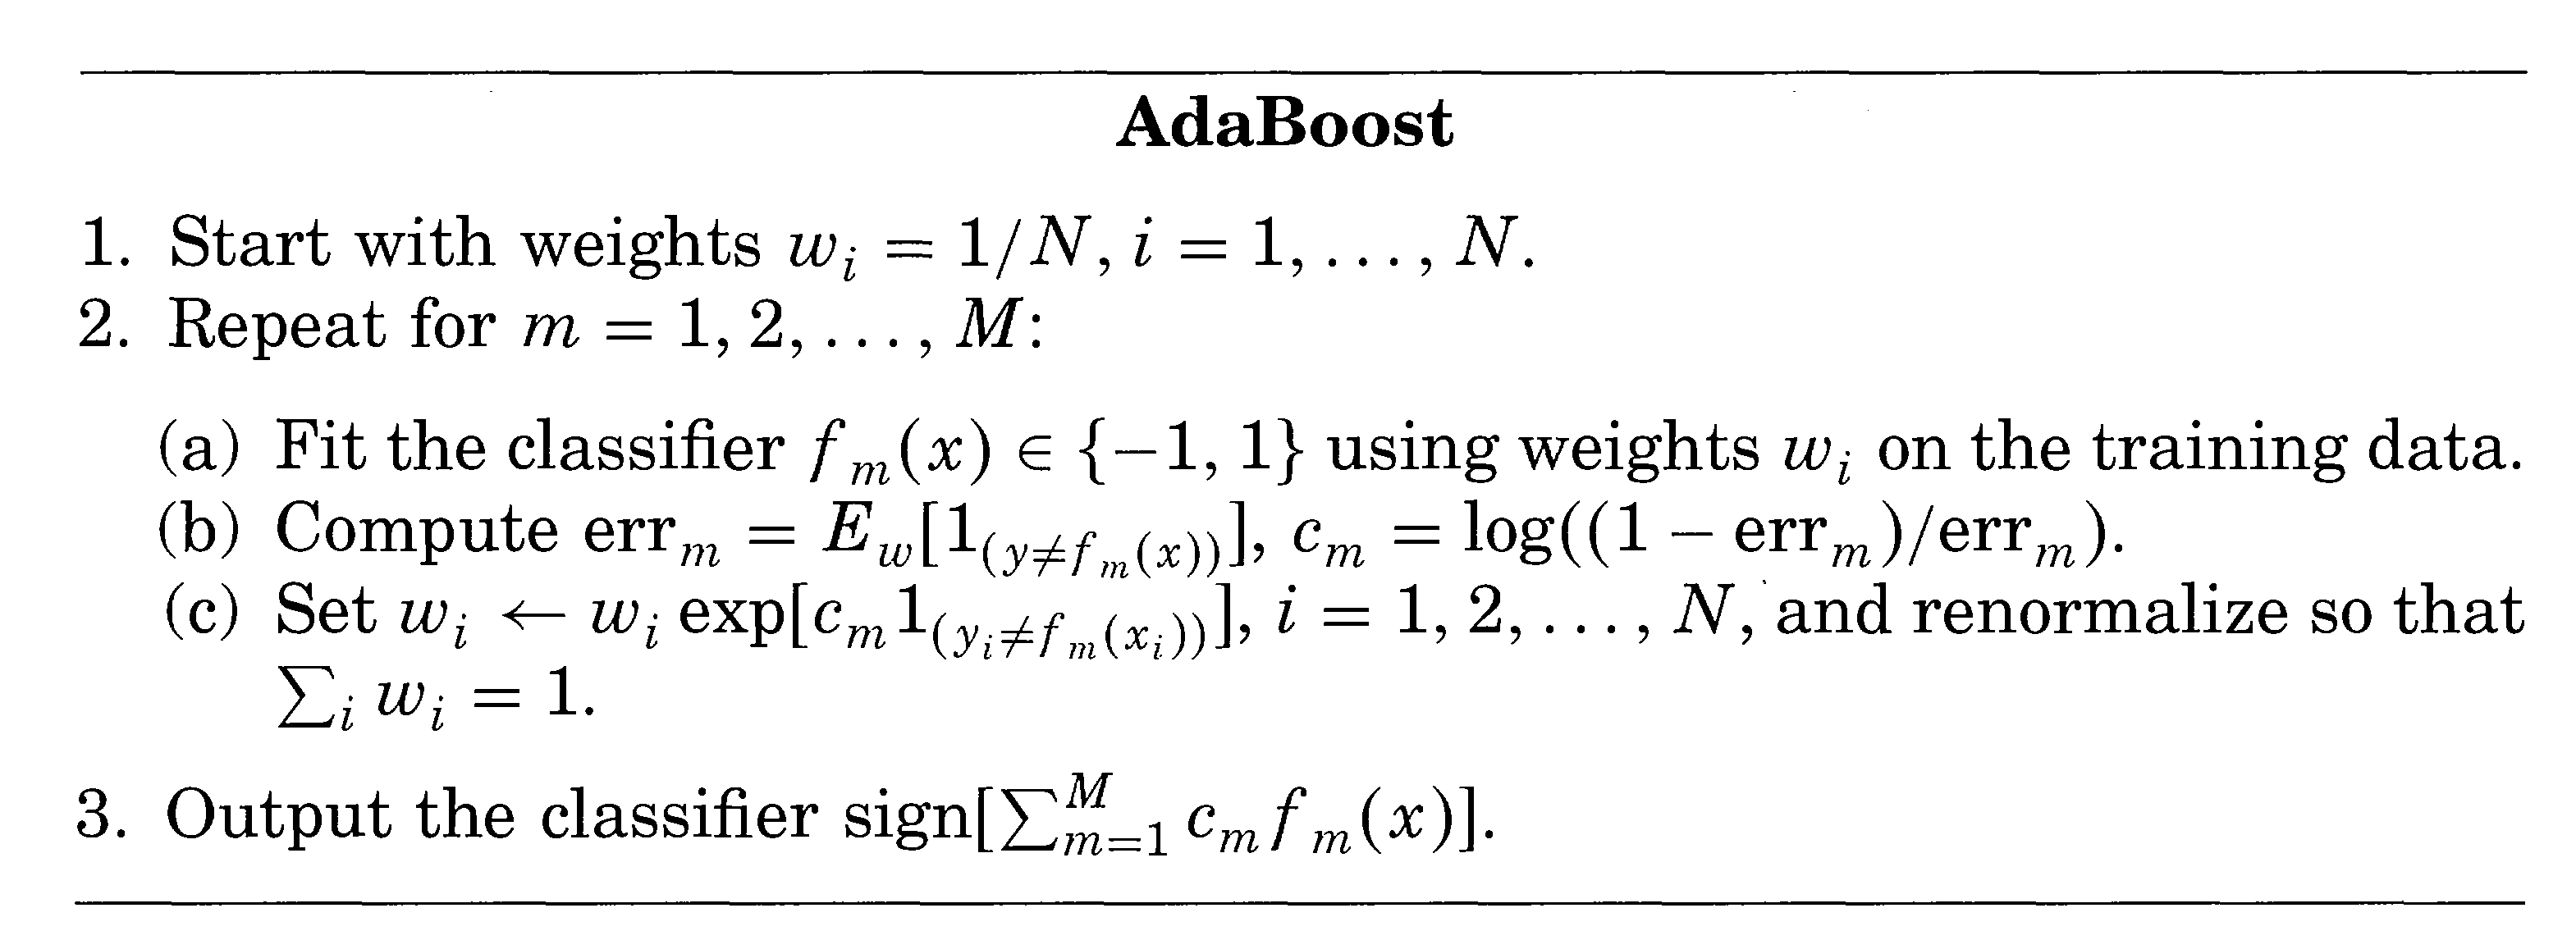
\includegraphics[width=0.8\textwidth]{ada.png}
\caption{AdaBoost algorithm. $E_w$ represents expectation over the training data with weights $w=(w_1,w_2,\ldots,w_N)$ and $I_{(S)}$ is the indicator of the set $S$~\cite{alr00}.}
\label{fig:adaproc}
\end{figure}

We used ``Stumps'' as weak learners. Stumps are single-split trees with only two terminal nodes. Stumps are simple to implement, typically have low variance and success of boosting depends on variance reduction~\cite{alr00}.

\subsubsection{Madlib Implementation}
The challenge in implementing (binary) Adaptive Boosting classification for MADlib is that, the algorithm is iterative in nature and in each iteration, it needs to make a pass over the entire training dataset as well as the weights data. Therefore, it cannot be implemented as a simple user-defined aggregate (UDA). We implemented AdaBoost as a driver UDF in Python. For performing Matrix arithmetic we used the {\ttfamily numpy} package. The control flow of the UDF is shown in Figure~\ref{fig:adaimp}.

\begin{figure}[h]
\centering
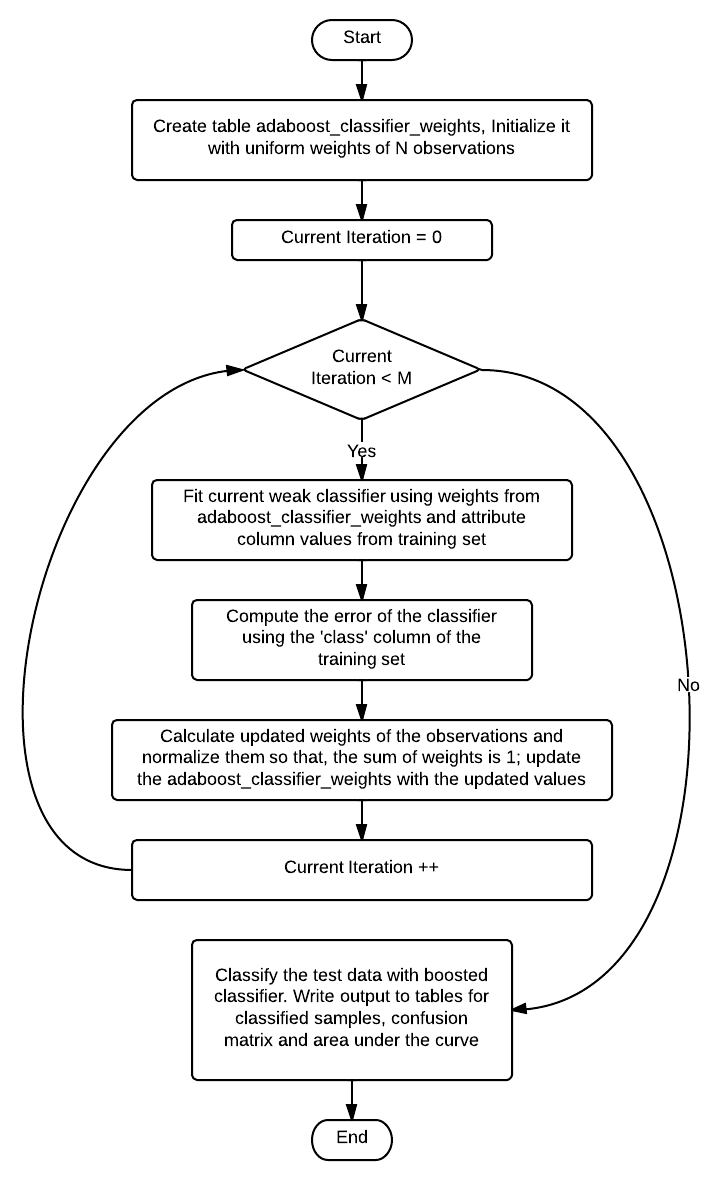
\includegraphics[scale=0.5]{adaimp.png}
\caption{Control Flow of AdaBoost Implementation for MADlib.}
\label{fig:adaimp}
\end{figure}

The row-by-row, batched and in-memory versions differ only in how we access the training and test dataset and weights table. See Appendix E for documentation of usage of AdaBoost module.



 

\section{Benchmark}
\label{sec:bench}
In this section, we show the results of the benchmarks that we performed to assess the performance of our implementations in various settings. We also discuss the implications of the results that we found.
\subsection{Setup}
We ran the benchmark on PostgreSQL 9.1.9 and MADlib v0.3 on a single machine on a gigabit Ethernet cluster which runs Ubuntu 12.04 LTS and has 4GB RAM, a 10GB SATA HDD and a Core 2 Duo 2.4GHz CPU. 

To benchmark the performance of GP for Symbolic Regression we used a synthetic dataset containing 100,000 rows, 3 inputs and 1 output. The function we used to generate the data is $x_1*(x_2^2+x_3)$.

To benchmark the performance of AdaBoost, we used BUPA liver disorder dataset which contains blood test results of 345 male individuals. This dataset is available at \url{http://www.cs.huji.ac.il/~shais/datasets/ClassificationDatasets.html}. We also used a synthetic dataset which consisted of $240000\times11$ matrix where first 10 columns are real valued random numbers and the last column indicates the class.

Each run of our algorithms inside MADlib was cold start meaning that we cleared the caches and restarted the database service (PostgreSQL) for every run.


%\subsection{Results}
%Tables~\ref{tab:gp}, \ref{tab:adaBupa1}, \ref{tab:adaBupa2}, \ref{tab:adaSynth1} and \ref{tab:adaSynth2} in Appendix A summarize our benchmark results. Table~\ref{tab:gp} shows <Filled by Franck>. In Table~\ref{tab:adaBupa1}, we record the runtimes of row-by-row execution, batched execution and all-in-memory execution of AdaBoost inside MADlib. In Table~\ref{tab:adaBupa2}, we record the runtimes of the same algorithm when it reads data from a file or from PostgreSQL database outside MADlib or loads data into memory from Postgres residing inside MADlib. In all cases we varied the number of iterations parameter. Table~\ref{tab:adaSynth1} shows the runtimes and Table~\ref{tab:adaSynth2} shows the memory usage of row-by-row execution, batched execution and all-in-memory execution of AdaBoost when it is run on a synthetic dataset of varying size.    

%As we can see from the tables, the runtime of both of the algorithms increases as we increase the number of independent variables. Running the algorithms using MADlib takes more time than bypassing MADlib altogether when data can be fit into memory. Running the algorithms using MADlib is advantageous when the dataset cannot be fit into memory. Batched execution is more efficient in terms of run time than row by row execution in terms of run time. It is more efficient than reading the whole dataset into memory in terms of memory usage.

\subsection{Analysis of Results}
Our benchmarking results are tabulated in Appendix A. Here, we discuss our understanding of the findings.

\subsubsection*{Effect of varying independent variables on runtime and memory usage.}
The first focus of our analysis was the effect of the parameters of the symbolic regression and of AdaBoost on runtime and memory usage. Figure \ref{fig:gp-inside-vs-outside} shows that when we increase the value of our parameters, it increases the runtime proportionally as expected. By the same token,  increasing the size of the data set cause PostgreSQL to use a higher amount of memory (Figure~\ref{fig:adamem} all-in-memory execution).

\begin{figure}[ht]
\centering
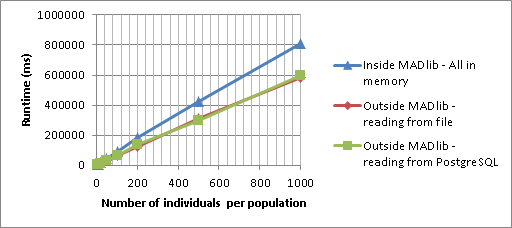
\includegraphics[width=0.8\textwidth,height=180px]{gp-inside-vs-outside.png}
\caption{Runtimes of symbolic regression inside and outside MADlib.}
\label{fig:gp-inside-vs-outside}
\end{figure}

\begin{figure}[ht]
\centering
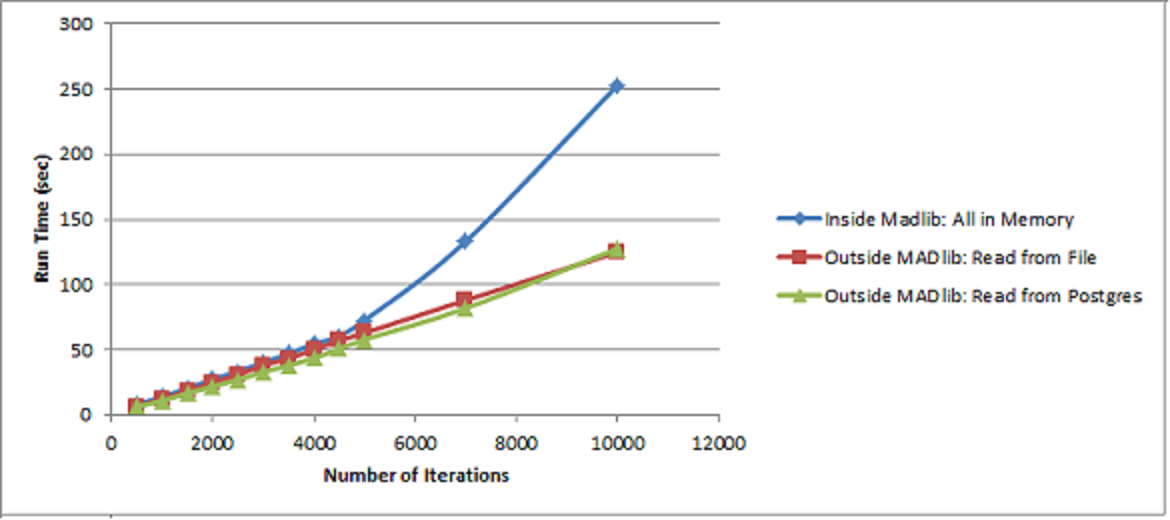
\includegraphics[width=0.8\textwidth,height=180px]{ada1.png}
\caption{Runtimes of AdaBoost algorithm inside and outside MADlib.}
\label{fig:adainout}
\end{figure}

\subsubsection*{Performance inside and outside MADlib}
Figure \ref{fig:gp-inside-vs-outside} also compares the runtime between different execution environments: within MADlib, outside MADlib reading from a file and outside MADlib reading from the PostgreSQL database. The code used in all the cases was strictly identical in order to ensure a fair comparison between execution environments. Also, all the data was loaded in memory just before the function call.

~~\\
First of all, in the case of the dataset that we used to perform symbolic regression, which contains 100,000 rows and of size 2686 KB, on average reading from a file takes 230 ms whereas it takes 510 ms reading from the PostgreSQL database. It takes 12.14 ms on average to read the BUPA dataset ($345\times7$) from file where reading from PostgreSQL takes 12.68 ms.

~~\\
The most intriguing result is the runtime within MADlib, which is significantly slower than the runtime outside MADlib. This result cannot be explained by the fact that querying the database makes running within MADlib slower since running outside MADlib reading from the PostgreSQL doesn't have the issue, and the difference of runtime increases when the number of iterations increases, which means the reason isn't a fixed cost.

~~\\
To investigate this difference of runtime we bypassed MADlib and created PL/Python test case that narrows down the issue:

\begin{verbatim}
CREATE FUNCTION testcase (b integer)
  RETURNS float
AS $$
  import time
  start = time.time()
  a = 0
  for i in range(b):
    for ii in range(b):
      a = (((i+ii)%100)*149819874987)
  end = time.time()
  plpy.info("Time elapsed in Python: " + str((end - start)*1000) + ' ms')
  return a
$$ LANGUAGE plpythonu;
\end{verbatim}

We compared the latter code with the following identical Python code:
\begin{verbatim}
import time
import sys

def testcase (b):     
    a = 0
    for i in range(b):
        for ii in range(b):
            a = (((i+ii)%100)*149819874987) # keeping Python busy
    return a

def main():    
    numIterations = int(sys.argv[1])        
    start = time.time()
    print testcase(numIterations)
    end = time.time()
    print "Time elapsed in Python:"
    print str((end - start)*1000) + ' ms'        

if __name__ == "__main__":
    main()
\end{verbatim}

~~\\
On our benchmark server, calling the PostgreSQL PL/Python function using \textit{select * from testcase(20000);}, it takes on average 65 seconds, while when we call the usual Python script with 20000 as argument too it takes an average 48 seconds. The averages were computed running the queries and scripts 10 times. This result means that for some reason the CPython that is embedded in PostgreSQL 9.1 is slower than the Python 2.7.3 we use outside PostgreSQL.

~~\\
We tested with PostgreSQL 9.2 (with Ubuntu 12.10 this time), and we still notice a runtime difference on my server (although overall 10\% faster, probably due to some new version of CPython). We also tried using plpython3u, which implements PL/Python based on the Python 3 language variant. plpythonu that we used before is equivalent to plpython2u, which implements PL/Python based on the Python 2 language variant. Using plpython3u is far slower (88 seconds), but when running the Python script using python3 it is also slower (75 seconds), although still significantly faster than plpython3u.

~~\\
TODO: try on my VM and conclude


\subsubsection*{Performance of batched execution.}

So far our modules have loaded all the data in memory, then performed the computations on them. However, in some situation we might not have enough memory to store all the data. In older to circumvent this issue our modules allow to define the amount of memory the user wants to grant to the module. To do so, our GP implementation lets the user to choose the batch size, which corresponds to the number of rows the module can put in memory and the AdaBoost implementation lets the user to choose the number of batches (dataset will be divided into the number of partitions chosen by the user). At each iteration of the algorithm, we retrieve data in batches. Since we cannot store them in memory, it means we will have in total a significant amount of read/write accesses to the database. The smaller the batch size the higher the amount of read/write queries at each iteration will be.

~~\\
Figure \ref{fig:gp-batch-histo} shows the effect of the batch size in the case of the symbolic regression. We fixed the parameters and only changed the batch size. As we can see, having a batch size of 10,000 rows or a batch size of 1,000 rows is a pretty good trade-off: for batch size = 10,000 rows, the runtime is 1.5  times bigger, and for batch size = 1,000 rows, the runtime a bit less than twice bigger. TODO: add reference to the table in the appendix. Since the memory used is proportional to the batch size, it makes using large batches look attractive. However, if we further decrease the batch size, we see that it starts having a very negative impact on the runtime. Figures \ref{fig:ada2} and \ref{fig:ada3} show similar impact on runtime due to batching when the number of iterations of AdaBoost algorithm increases.

\begin{figure}[ht]
\centering
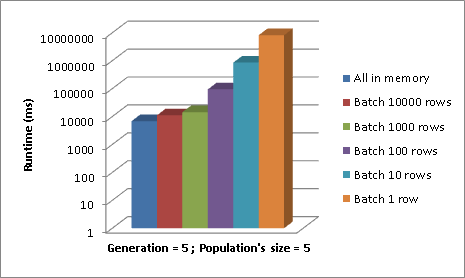
\includegraphics[width=0.8\textwidth,height=180px]{gp-batch-histo.png}
\caption{Runtimes of row-by-row, batched and all-in-memory execution of symbolic regression. The dataset contains 100,000 rows. Having a batch size of 10,000 rows means that at each iteration we do $100,000/10,000 = 10$ queries on the database}
\label{fig:gp-batch-histo}
\end{figure}

\begin{figure}[ht]
\centering
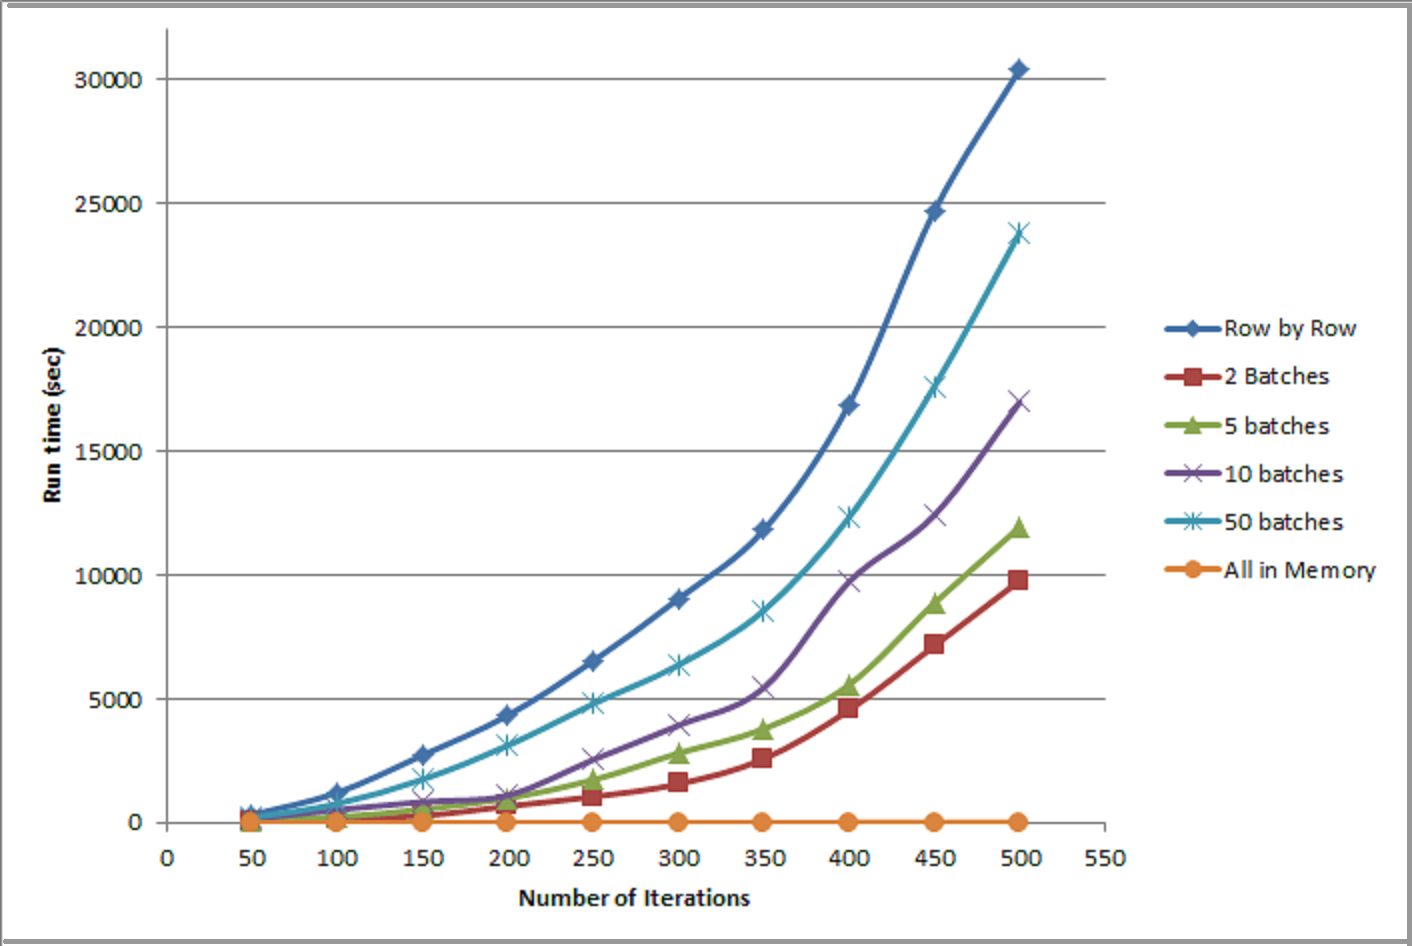
\includegraphics[width=0.8\textwidth,height=180px]{ada2.png}
\caption{Runtimes of row-by-row, batched and all-in-memory execution of AdaBoost algorithm on BUPA liver disorder dataset.}
\label{fig:adabatch1}
\end{figure}

\begin{figure}[ht]
\centering
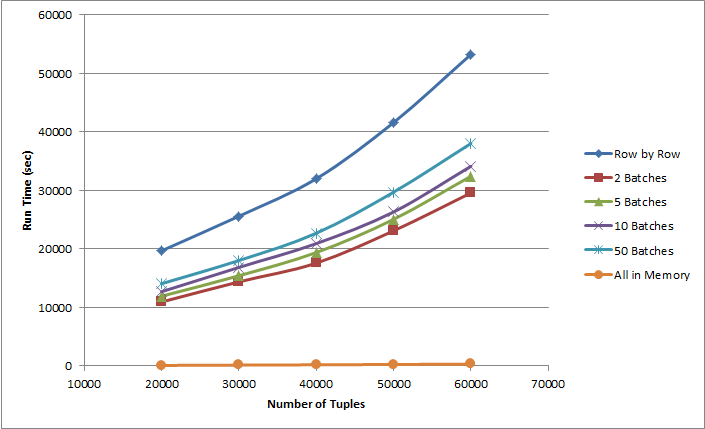
\includegraphics[width=0.8\textwidth,height=180px]{ada3.png}
\caption{Runtimes of row-by-row, batched and all-in-memory execution of AdaBoost algorithm on synthetic dataset.}
\label{fig:adabatch2}
\end{figure}

\begin{figure}[ht]
\centering
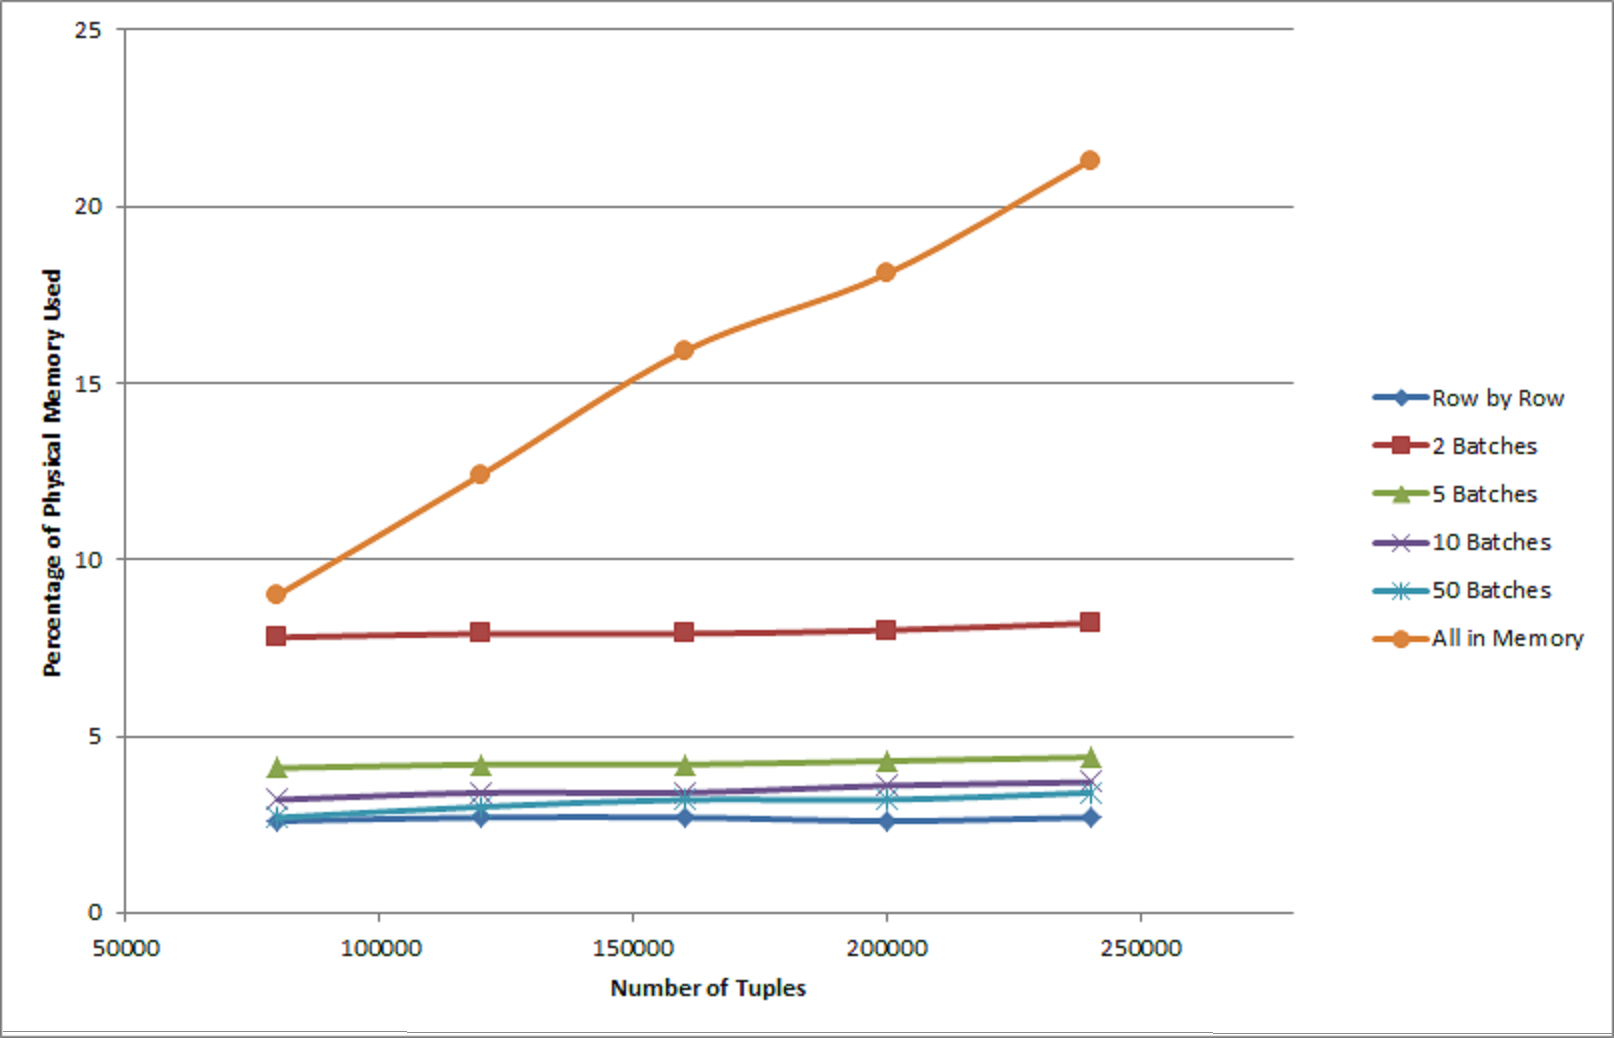
\includegraphics[width=0.8\textwidth,height=180px]{ada4.png}
\caption{Memory usage by AdaBoost algorithm on synthetic dataset.}
\label{fig:adamem}
\end{figure}

~~\\
Table~\ref{tab:adaSynth1} shows the runtimes and Table~\ref{tab:adaSynth2} shows the memory usage of row-by-row execution, batched execution and all-in-memory execution of AdaBoost when it is run on a synthetic dataset of varying size. We can see that, batching gives us advantage in terms of memory usage.




 

\section{Conclusions \& Future Work}
\label{sec:con}


\bibliographystyle{plain}
\bibliography{report}
\pagebreak
\section*{Appendix A: Tables showing Benchmarking Results}

\begin{table}[!htbp]
\centering
\begin{tabular}{lcc}
\end{tabular}
\caption{GP runtimes on synthetic dataset}
\label{tab:gp}
\end{table}

\begin{table}[!htbp]
\small
\centering
\begin{tabular}{|c|c|c|c|c|c|c|}
\hline
\multirow{2}{*}{NumIter} & \multicolumn{6}{|c|}{Runtimes (sec)}\\
\cline{2-7}
& All-in-Memory & 2 Batches & 5 Batches & 10 Batches & 50 Batches & Row-by-Row\\
\hline
50 &1.04 &96.72 &99.23 &149.96 &213.31 &314.75 \\
\hline
100 &2.09 &147.90 &236.93 &527.41 &770.55 &1215.30 \\
\hline
150 &2.69 &283.44 &548.98 &844.80 &1746.58 &2727.17 \\ 
\hline
200 &3.39 &675.45 &986.81 &1107.41 &3118.15 &4334.23 \\ 
\hline
250 &4.18 &1052.99 &1728.76 &2546.37 &3118.154 &6525.33 \\ 
\hline
300 &4.88 &1566.79 &2814.76 &3926.46 &6367.52 &9041.89 \\ 
\hline
350 &5.72 &2578.63 &3789.65 &5444.76 &8567.15 &11822.67 \\ 
\hline
400 &6.58 &4548.88 &5567.59 &9720.97 &12319.85 &16878.20 \\ 
\hline
450 &7.58 &7143.48 &8869.80 &12414.58 &17613.34 &24683.87 \\ 
\hline
500 &7.96 &9776.36 &11934.97 &16977.72 &23814.81 &30417.70 \\
\hline
\end{tabular}
\caption{AdaBoost runtimes on BUPA liver disorder dataset (Row-by-Row vs. Batched vs. All-in-Memory execution).}
\label{tab:adaBupa1}
\end{table}

\begin{table}[!htbp]
\small
\centering
\begin{tabular}{|c|c|c|c|}
\hline
\multirow{3}{*}{NumIter}&\multicolumn{3}{|c|}{Runtimes (sec)}\\
\cline{2-4}
&Outside MADlib&Outside MADlib&\multirow{2}{*}{Inside MADlib}\\
&from PostgreSQL&from File&\\
\hline
500&6.73 &6.37 &7.96 \\
\hline
1000&10.85 &12.23 &14.01 \\\hline
1500&16.82 &18.27 &20.43 \\\hline
2000&21.87 &24.56 &27.50 \\\hline
2500&27.13 &30.92 &33.52 \\\hline
3000&32.95 &38.25 &40.27 \\\hline
3500&38.11 &43.28 &47.11 \\\hline
4000&43.51 &50.45 &54.48 \\\hline
4500&50.86 &57.02 &60.51 \\\hline
5000&57.86 &62.97 &72.63 \\\hline
7000&82.00 &88.12 &133.256 \\\hline
10000&127.60 &124.88 &252.98 \\
\hline
\end{tabular}
\caption{AdaBoost runtimes on BUPA liver disorder dataset (Inside vs. Outside MADlib).}
\label{tab:adaBupa2}
\end{table}

\begin{table}[!htbp]
\small
\centering
\begin{tabular}{|c|c|c|c|c|c|c|}
\hline
\multirow{2}{*}{NumTuples} & \multicolumn{6}{|c|}{Runtimes (sec)}\\
\cline{2-7}
& All-in-Memory & 2 Batches & 5 Batches & 10 Batches & 50 Batches & Row-by-Row\\
\hline
20000&92.02 &10938.07 &11932.44 &12702.27 &14063.23 &19688.52 \\
\hline
30000&143.13 &14379.26 &15418.72 &16838.87 &18024.70 &25595.08 \\
\hline
40000&201.38 &17579.04 &19390.21 &20911.01 &22690.67 &31993.85 \\
\hline
50000&252.59 &23106.67 &25055.43 &26324.06 &29708.58 &41592.01 \\
\hline
60000&320.38 &29576.54 &32432.05 &34126.77 &38026.98 &53237.77 \\
\hline
\end{tabular}
\caption{AdaBoost runtimes on synthetic dataset.}
\label{tab:adaSynth1}
\end{table}

\begin{table}[!htbp]
\small
\centering
\begin{tabular}{|c|c|c|c|c|c|c|}
\hline
\multirow{2}{*}{NumTuples} & \multicolumn{6}{|c|}{Memory Usage (\%)}\\
\cline{2-7}
& All-in-Memory & 2 Batches & 5 Batches & 10 Batches & 50 Batches & Row-by-Row\\
\hline
80000& 9.0&7.8&4.1 &3.2 &2.7&2.6 \\
\hline
120000& 12.4&7.9 &4.2 &3.4&3.0 &2.7 \\
\hline
160000& 15.9&7.9 &4.2 &3.4 &3.2 &2.7 \\
\hline
200000& 18.1&8.0 &4.3 &3.6 &3.2 &2.6 \\
\hline
240000& 21.3&8.2 &4.4 &3.7 &3.4 &2.7 \\
\hline
\end{tabular}
\caption{AdaBoost memory usage for synthetic dataset}
\label{tab:adaSynth2}
\end{table}


\begin{table}[!htbp]
\small
\centering
\begin{tabular}{|c|c|c|c|c|}
\hline
\multirow{3}{*}{Pop size} & \multirow{3}{*}{\# of gen.} & \multicolumn{3}{|c|}{Runtimes (sec)}\\
\cline{3-5}
& &Outside MADlib&Outside MADlib&\multirow{2}{*}{Inside MADlib}\\
& &from PostgreSQL&from File&\\
\hline
5 & 5 & 5.513 & 4.860 & 6.787 \\ \hline
10& 5 & 7.166 & 6.295 & 8.560 \\\hline
20& 5 & 13.879 & 12.484 & 17.610 \\\hline
50& 5 & 32.568 & 30.637 & 44.261 \\\hline
100& 5 & 65.385 & 62.013 & 88.910 \\\hline
200& 5 & 135.105 & 128.238 & 182.672 \\\hline
500& 5 & 300.677 & 314.149 &425.092 \\\hline
1000& 5 & 597.274 &582.635 &810.041 \\\hline
5& 10 & 7.888 & 7.669& 10.523 \\\hline
5& 20 & 11.245 & 11.137 & 16.282 \\\hline
5& 50 & 25.119 & 23.975 & 35.220 \\\hline
5& 100 & 47.355 & 46.355 & 69.156 \\\hline
5& 200 & 92.778 & 95.063 & 119.511 \\\hline
5& 500 & 226.639 & 239.827 & 293.664 \\\hline
5& 1000 & 491.201 & 489.361 & 591.823 \\\hline
20& 20 & 44.813 & 44.813 & 56.965 \\
\hline
\end{tabular}
\caption{Symbolic Regression runtimes on synthetic dataset.}
\label{tab:GPruntimes}
\end{table}


\begin{table}[!htbp]
\small
\centering
\begin{tabular}{|c|c|c|c|c|c|c|}
\hline
\multirow{2}{*}{Pop; Gen} & \multicolumn{6}{|c|}{Runtimes (sec)}\\
\cline{2-7}
& All-in-Memory & 10000-row batch & 1000-row batch & 100-row batch & 10-row batch & Row-by-Row \\
\hline
5; 5 & 6.787 & 11.012 & 14.220 &  93.387 & 845.325 &8153.139 \\
\hline
\end{tabular}
\caption{Symbolic Regression runtimes on synthetic dataset. Pop stands for population size. Gen stands for number of generations.}
\label{tab:GPbatchRunTimes}
\end{table}



\section*{Appendix B: Installing Madlib with PostgreSQL}
The following instructions have been tested on Ubuntu 12.04 x64. They will not work with Ubuntu 12.04 x32 (MADlib does not have support for Ubuntu 32-bit). Also, MADlib doesn't work with GCC 4.7.*. Since,  Ubuntu 12.10 ships with GCC 4.7.2 it might be an issue while installing MADlib on Ubuntu 12.10.

\vspace{\baselineskip}
{\raggedleft Install PostgreSQL packages:}
\begin{verbatim}
$ sudo apt-get -y install \
  postgresql-9.1 libpq-dev \
  postgresql-server-dev-9.1 \
  postgresql-plpython-9.1
\end{verbatim}

{\raggedleft Download MADlib from \url{http://madlib.net} and copy .tar file to server:}
\begin{verbatim}
$ wget https://github.com/madlib/madlib/zipball/v0.5.0
$ unzip v0.5.0
$ cd madlib-madlib-5fabd88
\end{verbatim}

{\raggedleft Build Madlib:}
\begin{verbatim}
$ sudo apt-get -y install cmake
$ sudo apt-get -y install m4 gcc-4.6 g++-4.6 g++
$ ./configure
$ cd build/
$ make
$ make doc
$ make install
\end{verbatim}

{\raggedleft Connect to the database:}
\begin{verbatim}
$ sudo su - postgres
$ psql
\end{verbatim}

{\raggedleft Add a password to a role:}
\begin{verbatim}
postgres=# ALTER ROLE postgres WITH PASSWORD 'postgres';
\end{verbatim}

{\raggedleft Register Madlib with the PostgreSQL database}
\begin{verbatim}
$ /usr/local/madlib/bin/madpack -p postgres -c \ 
  \$USER@\$HOST/postgres install
\end{verbatim}

{\raggedleft Test the installation by running install check procedure:}
\begin{verbatim}
$ /usr/local/madlib/bin/madpack -p postgres -c \
  \$USER@\$HOST/\$DATABASE install-check
\end{verbatim}

\section*{Appendix C: Creating a module in Madlib}

Create a new function testpy. We are going to create this section in any module called 'testmod'.

\begin{itemize}
  \item Add new module folder: ./src/ports/postgres/modules/testmod/
  \item Create in this folder the following files:

\begin{itemize}
  \item \_\_init\_\_.py\_in  
  \item testmod.py\_in
  \item testmod.sql\_in
\end{itemize}

\item Modify ./src/config/Modules.yml and add a new line "	- name: testmod"
  \item recompile MADlib: with any user:

\begin{itemize}
  \item ./configure
  \item make install      \# (no need for make clean) (in the MADlib build folder)
\end{itemize}
  \item re-register MADlib into Postgresql (with postgres user):
  \begin{itemize}
  \item  /usr/local/madlib/bin/madpack -p postgres -c \$USER@\$HOST/postgres reinstall
  \end{itemize}
 \end{itemize}
 


\section*{Appendix D: How to use Genetic Programming module in MADlib}
\subsection*{Input}
The input data is expected to be of the following form:
\begin{verbatim}
TABLE tableName (
    x1 DOUBLE PRECISION,
    ...
    xN DOUBLE PRECISION,
    y DOUBLE PRECISION
)
\end{verbatim}

\subsection*{Usage}
Perform Symbolic Regression using Genetic Programming:
\begin{verbatim}
postgres=# SELECT * FROM madlib.gp (
               'inputTableName', 
               '{x1, ..., xN}', '{y}', 
                numIndividuals, 
                numGenerations, 
                maxDepthOfTree
           );
\end{verbatim}

\subsection*{Example}
This is an example showing how to perform symbolic regression using the genetic programming module in MADlib. 

\vspace{\baselineskip}
{\raggedleft Generate an artificial dataset using MATLAB that contains 100,000 rows:}

\lstset{language=Matlab}
\lstset{tabsize=4}
\begin{lstlisting}
x1 = 1:0.0001:(10+5000);
x2 = 10:0.0001:(19+5000);
x3 = 5:0.0001:(14+5000);
a =[x1; x2; x3; x1.*(x2.^2+x3)];
csvwrite('mock.csv', a(1:100000, :))
\end{lstlisting}

{\raggedleft Import this dataset within PostgreSQL:}
\begin{verbatim}
postgres=# CREATE TABLE mock (X1 real, X2 real, X3 real, Y1 real);
postgres=# COPY mock FROM '/root/mock.csv' DELIMITERS ',' CSV;
\end{verbatim}

{\raggedleft Run the symbolic regression, with 100 individuals per population size, 20 generations, and to maximum size of the trees of 3. We take 3 attributes as input (x1, x2 and x3) and one attribute as output (y1):}

\begin{verbatim}
postgres=# SELECT * from madlib.gp('mock', '{x1, x2, x3}', '{y1}', 100, 20, 3);
\end{verbatim}

{\raggedleft The above query produces the following output:}
\begin{verbatim}
           individual            |      fitness
---------------------------------+-------------------
 [mul, add, mul, x2, x2, x3, x1] | 0.000442927237356
 [mul, add, mul, x2, x2, x3, x1] | 0.000442927237356
 [mul, add, mul, x2, x2, x3, x1] | 0.000442927237356
 [mul, add, mul, x2, x2, x3, x1] | 0.000442927237356
 [mul, add, mul, x2, x2, x3, x1] | 0.000442927237356
 [mul, add, mul, x2, x2, x3, x1] | 0.000442927237356
 [mul, add, mul, x2, x2, x3, x1] | 0.000442927237356
 [mul, add, mul, x2, x2, x3, x1] | 0.000442927237356
 [mul, add, mul, x2, x2, x3, x1] | 0.000442927237356
(9 rows)
\end{verbatim}

{\raggedleft Each row corresponds to one individual, i.e. one formula. In this example, all rows correspond to the formula $x_1*(x_2^2+x_3)$, which is what we wanted to find. The fitness reflects how accurate each individual is. The lowest the fitness, the most accurate the formula is.}


\section*{Appendix E: How to use AdaBoost module in MADlib}
\label{sec:adaapp}
Currently our implementation supports only binary classification.

\subsection*{Input}
The {\itshape training data} as well as {\itshape test data} is expected to be of the following form:

\begin{verbatim}
TABLE tableName (
    id INTEGER, // should be 1 indexed
    attribute1 DOUBLE PRECISION,
    ...
    attributeN DOUBLE PRECISION,
    class INTEGER // should be either 1 or -1
)
\end{verbatim}

\subsection*{Usage}
Perform AdaBoost classification loading the whole dataset into memory: (This type of execution is pretty fast when the dataset is small and fits into memory)

\begin{verbatim}
postgres=# SELECT * from madlib.adaboost_train_and_classify (
               'trainingSet', 'testSet', 
               '{attribute1, ..., attributeN}', 
               'class', numberOfIterations, pValue
           );
\end{verbatim}

When the dataset cannot be fit into memory, the user can use either batched or row-by-row version of AdaBoost.
\vspace{\baselineskip}
{\raggedleft Perform row-by-row version of AdaBoost classification:}

\begin{verbatim}
postgres=# SELECT * from madlib.adaboostRow_train_and_classify (
               'trainingSet', 'testSet', 
               '{attribute1, ..., attributeN}', 
               'class', numberOfIterations, pValue
           );
\end{verbatim}

{\raggedleft Perform batched version of AdaBoost classification:}

\begin{verbatim}
postgres=# SELECT * from madlib.adaboostBatch_train_and_classify (
               'trainingSet', 'testSet', 
               '{attribute1, ..., attributeN}', 
               'class', numberOfBatches,
                numberOfIterations, pValue
           );
\end{verbatim}

\subsection*{Example}
This is an over-simplified example of the in-memory execution of AdaBoost classification. Batched and row-by-row versions are similar.
\vspace{\baselineskip}
{\raggedleft The training and test data:}

\begin{verbatim}
postgres=# SELECT * from trainingSet;
 id | attr1 | attr2 | attr3 | class 
----+-------+-------+-------+--------
  1 |    85 |    92 |    45 |     1 
  2 |    85 |    64 |    59 |    -1 
  3 |    86 |    54 |    33 |     1 
  4 |    91 |    78 |    34 |     1 
  5 |    87 |    70 |    12 |    -1 
  6 |    98 |    55 |    13 |     1 
(6 rows)

postgres=# SELECT * from testSet;
 id | attr1 | attr2 | attr3 | class 
----+-------+-------+-------+--------
  1 |    95 |    82 |    15 |    -1 
  2 |    86 |    54 |    54 |     1 
  3 |    88 |    64 |    43 |     1 
  4 |    81 |    70 |    46 |     1 
  5 |    97 |    77 |    10 |    -1 
  6 |    88 |    65 |    12 |    -1 
(6 rows)
\end{verbatim}

{\raggedleft Perform AdaBoost classification:}

\begin{verbatim}
postgres=# SELECT * FROM madlib.adaboost_train_and_classify (
               'trainingSet', 'testSet', 
               '{attr1, attr2, attr3}', 
               'class', 50, 0.05
           );
\end{verbatim}

{\raggedleft The above query produces the following output summary:}

\begin{verbatim}
      result_table_name      
-----------------------------
 adaboost_classifier_weights
 adaboost_classified_samples
 adaboost_confusion_matrix
 adaboost_AUC
(4 rows)
\end{verbatim}

{\raggedleft Check the contents of the above tables to get the classification results:}

\begin{verbatim}
postgres=# SELECT * FROM adaboost_classifier_weights;

 id |     weight      
----+-----------------
 0  | 0.0492970944955
 1  |  0.161430043833
 2  |  0.225351747846
 3  |  0.225351747846
 4  |  0.190980668725
 5  |  0.147588697256
(6 rows)

postgres=# SELECT * FROM adaboost_classified_samples;

 row_id |     score      | predicted_class 
--------+----------------+-----------------
 0      |  12.3265804125 |               1
 1      | -12.2369378612 |              -1
 2      |  11.9033472397 |               1
 3      |  11.9033472397 |               1
 4      |  10.7171405001 |               1
 5      | -12.0688375328 |              -1
(6 rows)

postgres=# SELECT * FROM adaboost_confusion_matrix;

 tp | fp | fn | tn 
----+----+----+----
  2 |  2 |  1 |  1
(1 row)

postgres=# SELECT * FROM adaboost_AUC;

      auc       
----------------
 0.444444444444
(1 row)

\end{verbatim} 

\end{document}
